\documentclass[12pt]{article}
\usepackage[utf8]{inputenc}
\usepackage{amsmath}
\usepackage{subcaption}
\usepackage{float}
\usepackage{graphicx}
\usepackage{epstopdf}
\usepackage{lineno}
\usepackage{color}
\newcommand{\de}[1]{$\langle${{\color{cyan}\slshape{\bfseries DE:} #1}$\rangle$}}
\newcommand{\rz}[1]{$\langle${{\color{magenta}\slshape{\bfseries RZ:} #1}$\rangle$}}
\newcommand\dbyd[2]{\frac{\mathrm d{#1}}{\mathrm d{#2}}}
\newcommand{\R}{\mathcal{R}}

\setlength{\parindent}{4em}
\setlength{\parskip}{1em}
\renewcommand{\baselinestretch}{1.2}

\title{Intensional infect proportion of susceptible}

\begin{document}
\linenumbers
\maketitle
\section{Introduction}
Another approach would be to intentionally infect susceptible individuals, with a certain rate. Realistically, this approach is harder to achieve, since it takes extra resources to identify susceptible individuals inside a population. However, there has been examples in history. i.e. Chicken pox party.

\section{System of differential equations}
The following assumptions are made:
\begin{itemize}
\item There is no disease induced mortality.
\item Birth and natural death rate are the same, so the total population remains constant.
\item The latent period is short enough to be ignored.
\item All susceptible individuals are equally likely to be infected, and all infected individuals are equally infectious.
\end{itemize}

\begin{equation}\label{1}
\begin{split}
\dbyd{S}{t}&=\mu- \beta SI-rS-\mu S\,, \\
\dbyd{I}{t}&=rS+\beta SI-\gamma I -\mu I\,,\\
\dbyd{R}{t}&=\gamma I-\mu R\,,
\end{split}
\end{equation}

Where $\beta$ is transmission rate, $\gamma$ is recovery rate, $\mu$ is the \emph{per capita} rate of birth and death, $r$ is the rate of intensional infection on susceptible individuals. We will discuss the reasonable value of $r$ in later sections.

Once again, we convert our system into dimensionless form, using dimensionless time coordinate.

\begin{equation}
\tau=(\gamma+\mu)t\,,
\end{equation}

Therefore, the result of conversion is:
\begin{equation}
\begin{split}
\dbyd{S}{\tau}&=\epsilon- \R_0  SI-\eta S-\epsilon S\,, \\
\dbyd{I}{\tau}&=\eta S+\R_0 SI-I\,,\\
\dbyd{R}{\tau}&=(1-\epsilon)I-\epsilon R\,,
\end{split}
\end{equation}

Where $\epsilon=\frac{\mu}{\gamma+\mu}$, $\R_0=\frac{\beta}{\gamma+\mu}$, $\eta=\frac{r}{\gamma+\mu}$

\section{Endemic equilibrium}
To find the endemic equilibrium(EE), once again, we let all equations in (3) equal to 0, and solve for $S$ and $I$, what we get is the following:

\begin{align}
S &= \frac{1}{\R_0}-\frac{2\eta}{\R_0(-(\eta+\epsilon-\epsilon\R_0)+\sqrt{(\eta+\epsilon-\epsilon\R_0)^2+4\R_0\epsilon \eta}+2\eta)}\\
I &= \frac{-(\eta+\epsilon-\epsilon\R_0)+\sqrt{(\eta+\epsilon-\epsilon\R_0)^2+4\R_0\epsilon \eta}}{2\R_0}
\end{align}

To analyze the stability at EE we use Jacobian matrix, which is the following,
\begin{equation}
\mathcal{J} =
\begin{bmatrix}
    \ -\R_0 I-\eta-\epsilon       & -\R_0 S \\
    \ \eta+\R_0 I       & \R_0 S-1 \\
\end{bmatrix}\,.
\end{equation}

Again, for simplicity. Let 
\begin{equation}
G=-(\eta+\epsilon-\epsilon\R_0)+\sqrt{(\eta+\epsilon-\epsilon\R_0)^2+4\R_0\epsilon \eta}.
\end{equation}
Notice, $G>0$, if $\epsilon,\eta\neq 0$

So Jacobian at EE becomes,
\begin{equation}
\mathcal{J}|_{E.E.}=
\begin{bmatrix}
    \ \frac{G}{2}-\eta-\epsilon       & -1+\frac{2\eta}{G+2\eta} \\
    \ \eta+\frac{G}{2}       & -\frac{2\eta}{G+2\eta} \\
\end{bmatrix}\,.
\end{equation}

Thus, eigenvalues of of Jacobian are the following:

\begin{align}
\lambda_{1,2} &= \frac{-(G^2+4\eta G+2\epsilon G+4\eta^2+4\epsilon\eta+4\eta) }{4(G+2\eta)}\\
& \pm \frac{\sqrt{((G^2+4\eta G+2\epsilon G+4\eta^2+4\epsilon\eta+4\eta)^2-4(2G^3+12\eta G^2+24\eta^2 G+8\epsilon\eta G+16\eta^3+16\epsilon\eta^2)}}{4(G+2\eta)}
\end{align}

We know that $G>0$, and since the rate of intentional infection is non-zero, so $\eta >0$

Thus, the discriminant($\Delta$) satisfies the following inequality,
\begin{equation}
\Delta<|(G^2+4\eta G+2\epsilon G+4\eta^2+4\epsilon\eta+4\eta)|
\end{equation}

Therefore, we can conclude that Re($\lambda$)$<0$, thus EE is stable.

To understand the dynamics of the system, we still need to decide whether it is a damped oscillation or not, by determining the sign of the discriminant.

Now we want to analyze with specific values of each parameter. So once more, we are going to use smallpox.

The following values are used (need reference): 
\begin{enumerate}
\item With 50 years of average life span, $\mu=\frac{1}{50*365}$.
\item 22 days of mean infectious period, $\gamma=\frac{1}{22}$.
\item $\R_0=4.5$.
\end{enumerate}
Therefore, we can calculate $\epsilon=\frac{\mu}{\mu+\gamma}=0.0012$

\subsection{Dependence of discriminant on rate of intentional infection ($\eta$)}

By using the parameter listed above, $G=-(\eta-0.0042)+\sqrt{(\eta-0.0042)^2+0.0216\eta}$

\begin{align}
\lambda_{1,2} &= \frac{-(G^2+4\eta G+0.0024 G+4\eta^2+0.0048\eta+4\eta) }{4(G+2\eta)}\\
& \pm \frac{\sqrt{((G^2+4\eta G+0.0024 G+4\eta^2+0.0048\eta+4\eta))^2-4(2G^3+12\eta G^2+24\eta^2 G+0.0096\eta G+16\eta^3+0.0192\eta^2)}}{4(G+2\eta)}
\end{align}

So I plotted the discriminant using Mathematica, here is what I got:

\begin{figure}[h!]
  \caption{Plot discriminant with $\eta$ to be the variable.}
  \centering
  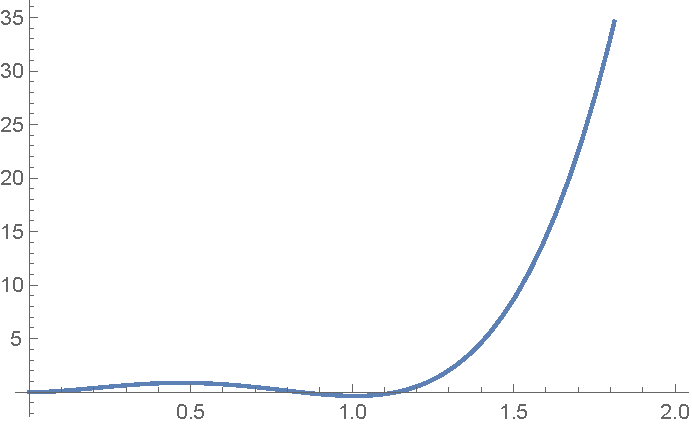
\includegraphics[width=1\textwidth]{Figures/Discriminant_plot_S.pdf}
\end{figure}

The $\eta$-intercept of this plot is $\eta_1=0.000704619$, $\eta_2=0.840164$, $\eta_3=1.13557$. The corresponding interpretations are: average time before being intentional infected are 31184.95, 26.15, 19.35 days, respectively.

Realistically, it should not take on average 85 years to intentionally infect an individual. so we can reject $\eta_1=0.000704619$.

Thus, if we are intentionally infecting slower than $\eta_2$ (on average 26.15 days before intentionally infected) or faster than $\eta_3$(n average 19.35 days), there is no damped oscillation, or otherwise there is.

For value of $\eta$, it is reasonable to assume the average number of days before an individual to be intentionally infected is between 30-60 days. Thus our range of $\eta$ could vary from 0.36623 - 0.73245. Thus, from this range, we should get a positive discriminant value, hence, there is no damped oscillation.

\subsection{Dependence of discriminant on basic reproduction number ($\R_0$)}

This time, I take $\mu=\frac{1}{50*365}$, $\gamma=\frac{1}{22}$, $\epsilon=\frac{\mu}{\mu+\gamma}=0.000753$. 

Now I take $\eta=0.4885$, as it correspond to the average number of days before an individual get intentionally infected being 45 days.

Again, I did the plot of discriminant.

\begin{figure}[H]
  \caption{Plot discriminant with $\R_0$ to be the variable.}
  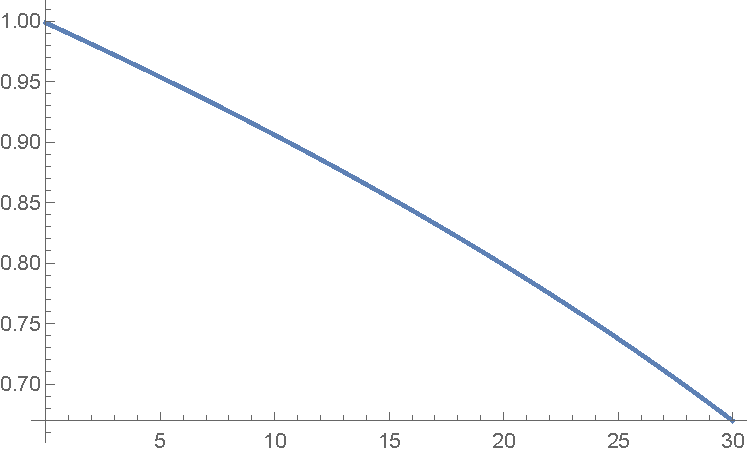
\includegraphics[width=1\textwidth]{Figures/Plot_R_S.pdf}
\end{figure}

The $\R_0$ intercept of this plot is $\R_0=52.439$, it is not in the range of reasonable value for $\R_0$.

The plotting result shows that discriminant is always positive,for a reasonable $\mathcal{R}_0$ value. Thus, if we take $\eta=0.4885$, there is never going to be a damped oscillation.

The value of discriminant is much more sensitive to $\eta$ than to $\mathcal{R}_0$.

\section{DFE}

Disease free equilibrium is the equilibrium when there is nobody infected in the system, which means, $I=0$

Again, we solve equations (3) by letting both $\dbyd{S}{\tau}$ and $\dbyd{I}{\tau}$ equal to 0. But this time, since it is disease free, $I=0$ as well.

Thus we have:
\begin{equation}
\dbyd{I}{\tau}=\eta S+\mathcal{R}_0 SI-I=\eta S=0
\end{equation}

This system only has a solution if $\eta=0$ or $S=0$. However, if $\eta=0$, this is again the basic SIR model, which we are not going to consider, thus $S=0$.

However, the other equation is now not satisfied. By substituting $S=0$ into $\dbyd{S}{\tau}$, we get:

\begin{equation}
\dbyd{S}{\tau}=\epsilon\neq0
\end{equation}

Consequently, we are able to conclude that disease free equilibrium does not exist for this model as well.

\section{I at E.E.}

\begin{figure}[H]
  \caption{I at E.E. as a function of $\R_0$, when $\eta=0.4883$}
  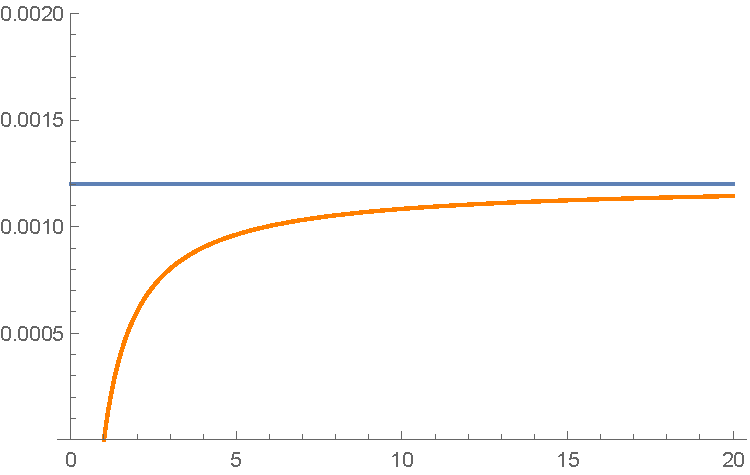
\includegraphics[width=1\textwidth]{Figures/Plot_I_at_EE_vary_R_0.pdf}
\end{figure}

As we can see from the scale of the vertical axis, $I_{E.E.}$ is not sensitive to the change of $\R_0$. But it is still higher than the normal SIR model.

To know how much $I|_{E.E.}$ has increased, it is helpful to see the ratio between $I_{E.E.}$ values for our model and basic SIR model.

\begin{figure}[H]
  \caption{Ratio between $I_{E.E.}$ values for our model and basic SIR model, as a function of $R_0$}
  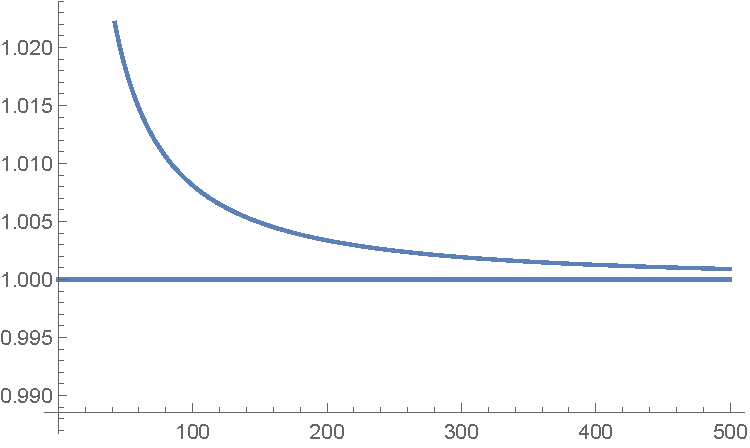
\includegraphics[width=1\textwidth]{Figures/Ratio_plot.pdf}
\end{figure}

As $\R_0$ increases, the ratio eventually approaches 1. But a reasonable range of $\R_0$, the ratio is still high.

\section{Conclusion}
\begin{flushleft}
Our models presented two different approaches of intentional infection. Both approaches are proven to have a stable endemic equilibrium, regardless of what value $\R_0$ has, which is different from basic SIR model, where E.E. is only stable if $\R_0>1$.

In these models, since we are not considering possible deaths caused by the disease, we are unable to conclude any advantages of this method whatsoever. However, previous research has reported significant decrease of death rate when performing variolation on smallpox (need reference). This could be our next step, to observe advantages of intentional infections, over normal SIR model or even vaccination models.

\end{flushleft}
\end{document}